\documentclass[11pt,aspectratio=169]{beamer}

\usepackage[utf8]{inputenc}
\usepackage[T1]{fontenc}
\usepackage[french]{babel}
\usepackage{lmodern}
\usepackage{graphicx}
\usepackage{amsmath,amssymb}
\usepackage{booktabs}

% --- Thème ---
\usetheme{Madrid}
\usecolortheme{whale}
\definecolor{bleu}{HTML}{1F4E79}
\definecolor{bleuc}{HTML}{2563EB}
\setbeamercolor{structure}{fg=bleu}
\setbeamertemplate{navigation symbols}{}
\setbeamertemplate{caption}[numbered]
\setbeamerfont{title}{size=\Large,series=\bfseries}
\setbeamertemplate{itemize item}{\color{bleuc}\textbullet}
\setbeamertemplate{itemize subitem}{\color{bleuc}--}

% --- Infos titre ---
\title[Snake évolutif (Sujet 2)]{Snake évolutif sur grille dynamique}
\subtitle{Un agent neuroévolutionnaire dans un environnement Gymnasium personnalisé}
\author[Benaqqa \& Bensmina]{Benaqqa Moubarak \and Bensmina Anass}
\institute[ENSIAS]{ENSIAS --- Module M2442 « Jeux Vidéo IA »}
\date{\today}

\begin{document}

% ===================== TITRE ===================== %
\begin{frame}[plain]
  \titlepage
\end{frame}

% ===================== PLAN ===================== %
\begin{frame}{Plan de la présentation}
  \begin{enumerate}
    \item Le problème et l'environnement
    \item L'agent et l'algorithme génétique
    \item Le protocole expérimental
    \item Les résultats
    \item Difficultés, limites et améliorations
  \end{enumerate}
\end{frame}

% ===================== 1. PROBLEME ===================== %
\section{Problème}

\begin{frame}{1. Le problème : Snake sur grille \emph{dynamique}}
  \begin{columns}
    \begin{column}{0.58\textwidth}
      \textbf{Objectif (Sujet 2)} : un serpent doit \textbf{manger un maximum
      de nourriture} tout en \textbf{survivant} sur une grille $12\times12$.
      \medskip
      \begin{itemize}
        \item Manger $\Rightarrow$ score $+1$, le serpent grandit
        \item Heurter mur / obstacle / son corps $\Rightarrow$ mort
        \item Ne pas manger trop longtemps $\Rightarrow$ famine
      \end{itemize}
      \medskip
      \textbf{« Dynamique » :} à chaque épisode, le nombre d'obstacles
      ($3$ à $10$) et le budget de survie \textbf{changent aléatoirement}.
    \end{column}
    \begin{column}{0.42\textwidth}
      \begin{block}{Pourquoi c'est intéressant}
        Pas de carte fixe à mémoriser : l'agent doit apprendre une
        \textbf{politique générale}, robuste à toutes les configurations.
      \end{block}
    \end{column}
  \end{columns}
\end{frame}

\begin{frame}{1. Environnement Gymnasium personnalisé}
  \begin{columns}
    \begin{column}{0.5\textwidth}
      \textbf{Actions (discrètes, relatives)}
      \begin{itemize}
        \item Tout droit / Tourner à droite / Tourner à gauche
        \item Élimine les demi-tours suicidaires
      \end{itemize}
      \medskip
      \textbf{Observation (11 valeurs)}
      \begin{itemize}
        \item Danger immédiat (3 directions)
        \item Direction courante (one-hot, 4)
        \item Position relative de la nourriture (4)
      \end{itemize}
    \end{column}
    \begin{column}{0.5\textwidth}
      \textbf{Récompense}
      \[
      r=\begin{cases}
        +1 & \text{manger}\\
        -1 & \text{collision}\\
        -0.5 & \text{famine}\\
        \pm0.1 & \text{(rapproch.\ nourriture)}
      \end{cases}
      \]
      \medskip
      \textbf{Fin d'épisode} : collision, famine, victoire (grille pleine)
      ou troncature.
      \medskip
      \footnotesize\textit{Signature respectée :}\\
      \texttt{(obs, reward, terminated, truncated, info)}
    \end{column}
  \end{columns}
\end{frame}

% ===================== 2. AGENT ===================== %
\section{Agent}

\begin{frame}{2. L'agent : neuroévolution}
  \textbf{Politique = petit réseau de neurones (MLP)}
  \[
  \text{obs}_{(11)} \;\to\; \tanh_{(16)} \;\to\; \text{logits}_{(3)} \;\xrightarrow{\arg\max}\; \text{action}
  \]
  \begin{itemize}
    \item \textbf{Génome} = les 243 poids du réseau (vecteur de réels)
    \item Pas de gradient : les poids sont optimisés par \textbf{algorithme génétique}
  \end{itemize}
  \vspace{0.3cm}
  \begin{block}{Fonction de fitness}
    \[
    \text{fitness} = \underbrace{100\,\bar{s}}_{\text{score (priorité)}}
    + \underbrace{0.5\,\bar{t}}_{\text{survie}}
    + \underbrace{\bar{R}}_{\text{récompense}}
    \]
    Évaluée sur plusieurs épisodes pour mesurer la \textbf{généralisation}.
  \end{block}
\end{frame}

\begin{frame}{2. L'algorithme génétique}
  \begin{columns}
    \begin{column}{0.55\textwidth}
      \textbf{Opérateurs}
      \begin{itemize}
        \item \textbf{Sélection} : tournoi (taille 5)
        \item \textbf{Croisement} : uniforme (gène par gène)
        \item \textbf{Mutation} : bruit gaussien, amplitude
              \textbf{décroissante} ($0.25 \to 0.10$)
        \item \textbf{Élitisme} : les 12\% meilleurs survivent intacts
      \end{itemize}
    \end{column}
    \begin{column}{0.45\textwidth}
      \begin{block}{Cycle évolutif}
        \footnotesize
        Évaluer $\to$ Sélectionner $\to$ Croiser $\to$ Muter $\to$ Remplacer
        \\[0.2cm]
        \normalsize
        Population : 150 individus\\
        Générations : 150
      \end{block}
    \end{column}
  \end{columns}
\end{frame}

% ===================== 3. PROTOCOLE ===================== %
\section{Protocole}

\begin{frame}{3. Protocole expérimental}
  \begin{itemize}
    \item \textbf{Deux baselines} de comparaison :
      \begin{itemize}
        \item Agent \textbf{aléatoire} (borne basse)
        \item Agent \textbf{heuristique} : évite le danger + va vers la
              nourriture (référence forte, codée à la main)
      \end{itemize}
    \item \textbf{Séparation stricte} entraînement / test : les 200 épisodes de
          test (graines $[900000,900199]$) ne sont \textbf{jamais vus} pendant
          l'évolution.
    \item Tous les agents évalués sur \textbf{exactement les mêmes épisodes}
          $\Rightarrow$ comparaison équitable et reproductible.
    \item \textbf{Indicateurs} : score moyen $\pm$ écart-type, score max,
          survie moyenne, taux de réussite, robustesse aux obstacles.
  \end{itemize}
\end{frame}

% ===================== 4. RESULTATS ===================== %
\section{Résultats}

\begin{frame}{4. L'agent apprend bien}
  \begin{figure}
    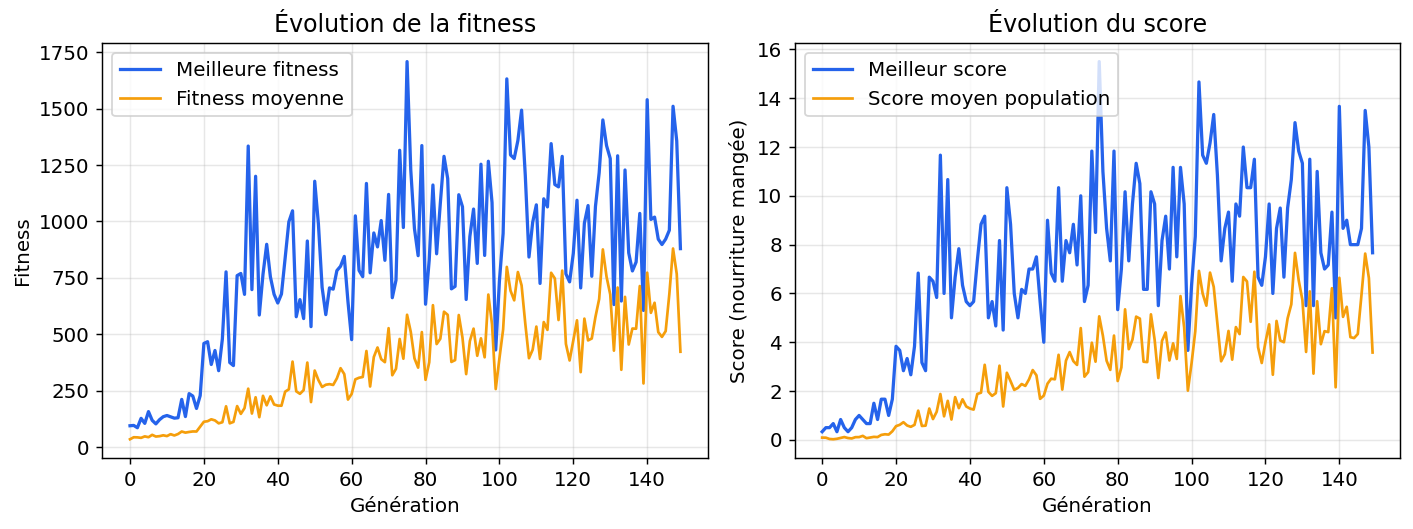
\includegraphics[width=0.92\textwidth]{fig_evolution.png}
  \end{figure}
  \centering
  \footnotesize Le score grimpe de $\approx 0$ à des pics $>13$ : l'évolution
  découvre une politique compétente \textbf{à partir de poids aléatoires}.
\end{frame}

\begin{frame}{4. Comparaison aux baselines (200 épisodes de test)}
  \begin{columns}
    \begin{column}{0.46\textwidth}
      \begin{table}
        \footnotesize
        \begin{tabular}{lcc}
          \toprule
          \textbf{Agent} & \textbf{Score} & \textbf{Survie} \\
          \midrule
          Aléatoire   & 0.09  & 15.4 \\
          \textbf{AG} & \textbf{6.30}  & \textbf{172.8} \\
          Heuristique & 15.97 & 153.1 \\
          \bottomrule
        \end{tabular}
      \end{table}
      \medskip
      \begin{itemize}
        \footnotesize
        \item AG : score $\times 70$ vs aléatoire
        \item AG \textbf{survit plus longtemps} que l'heuristique
        \item Reste sous l'heuristique en score
      \end{itemize}
    \end{column}
    \begin{column}{0.54\textwidth}
      \begin{figure}
        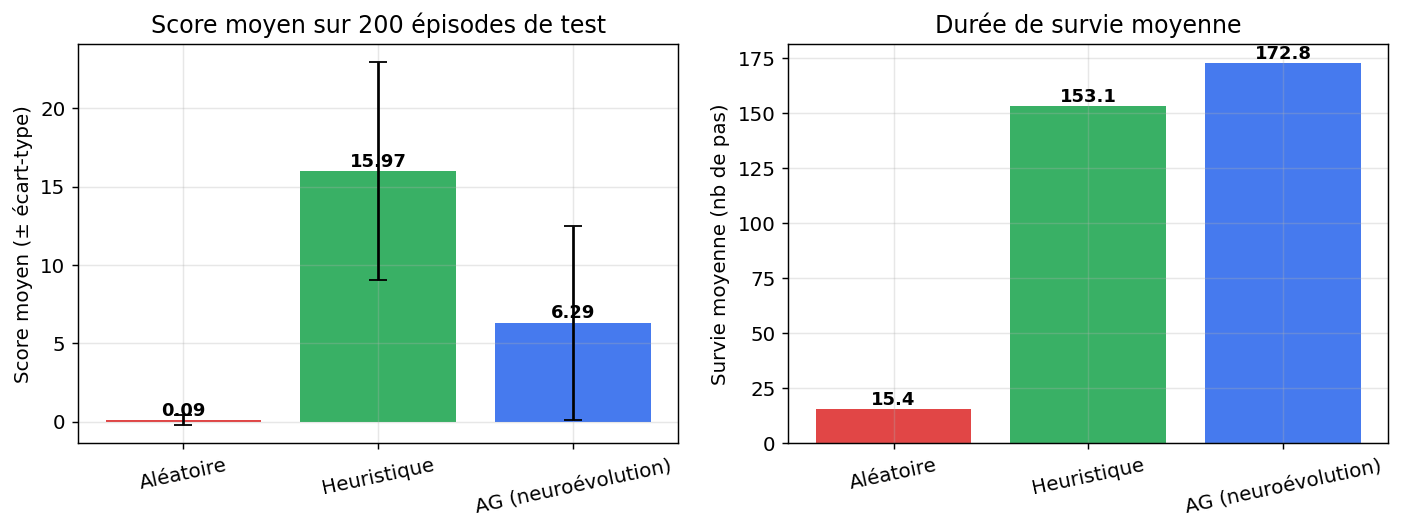
\includegraphics[width=\textwidth]{fig_comparaison.png}
      \end{figure}
    \end{column}
  \end{columns}
\end{frame}

\begin{frame}{4. Robustesse : où est la marge de progrès ?}
  \begin{columns}
    \begin{column}{0.55\textwidth}
      \begin{figure}
        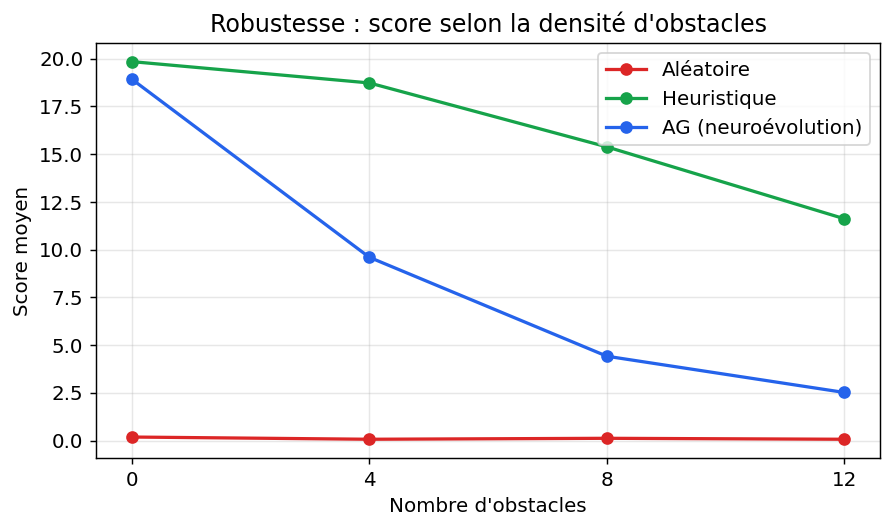
\includegraphics[width=\textwidth]{fig_robustesse.png}
      \end{figure}
    \end{column}
    \begin{column}{0.45\textwidth}
      \begin{block}{Diagnostic clé}
        \textbf{Sans obstacle}, l'AG ($18.9$) \textbf{égale presque}
        l'heuristique ($19.9$) !
        \medskip
        La recherche de nourriture est \textbf{excellente} ; c'est la
        \textbf{gestion des obstacles} qui le pénalise quand ils sont nombreux.
      \end{block}
    \end{column}
  \end{columns}
\end{frame}

% ===================== 5. LIMITES ===================== %
\section{Limites}

\begin{frame}{5. Difficultés, limites et améliorations}
  \begin{columns}
    \begin{column}{0.5\textwidth}
      \textbf{Limites identifiées}
      \begin{itemize}
        \item Vision \textbf{très locale} (1 case) : pas d'anticipation des
              impasses
        \item Fitness \textbf{bruitée} (épisodes aléatoires)
        \item Réseau et budget évolutif modestes
      \end{itemize}
    \end{column}
    \begin{column}{0.5\textwidth}
      \textbf{Pistes d'amélioration}
      \begin{itemize}
        \item Observation \textbf{enrichie} (vision sur plusieurs cases)
        \item Réduire le bruit (plus d'épisodes, graines communes)
        \item \textbf{CMA-ES} ou \textbf{NEAT} (topologie évolutive)
        \item \textbf{Curriculum} : difficulté croissante
      \end{itemize}
    \end{column}
  \end{columns}
\end{frame}

% ===================== CONCLUSION ===================== %
\begin{frame}{Conclusion}
  \begin{block}{Ce que nous avons réalisé}
    \begin{itemize}
      \item Un environnement Gymnasium \textbf{personnalisé} et \textbf{dynamique}
            pour le jeu Snake
      \item Un agent \textbf{neuroévolutionnaire} complet (MLP + AG : sélection,
            croisement, mutation, élitisme)
      \item Un protocole \textbf{rigoureux et reproductible} avec deux baselines
    \end{itemize}
  \end{block}
  \medskip
  \textbf{Résultat :} à partir de poids \emph{aléatoires} et sans aucune
  connaissance experte, l'évolution fait émerger une stratégie cohérente de
  recherche de nourriture et de survie (score $\times 70$ vs aléatoire,
  survie supérieure à l'heuristique).
\end{frame}

\begin{frame}[plain]
  \centering
  \vfill
  {\Huge\bfseries\color{bleu} Merci de votre attention}\\[0.8cm]
  {\large Questions ?}\\[1.2cm]
  {\normalsize Benaqqa Moubarak \quad\textbullet\quad Bensmina Anass}\\
  {\footnotesize ENSIAS --- M2442 « Jeux Vidéo IA »}
  \vfill
\end{frame}

\end{document}
